\documentclass[10pt,letterpaper,fleqn]{article}

\usepackage[utf8]{inputenc}
\usepackage[spanish,es-nodecimaldot]{babel}
\usepackage{amsmath}
\usepackage{amssymb}
\usepackage{multicol}
\usepackage{graphicx}
\usepackage{mdwlist}

\usepackage[dvipsnames]{xcolor}
\usepackage[most]{tcolorbox}

\usepackage{tabu}

\usepackage{mathtools}

\usepackage[top=1in, bottom=1in, left=1in, right=1in]{geometry}


\begin{document}

\begin{titlepage}
    \centering

    {\scshape\LARGE Universidad Nacional Autónoma de México \par}

    \vspace{1cm}
    {\scshape\Large Facultad de Ciencias\par}
    \vspace{1.5cm}

    \begin{center}
        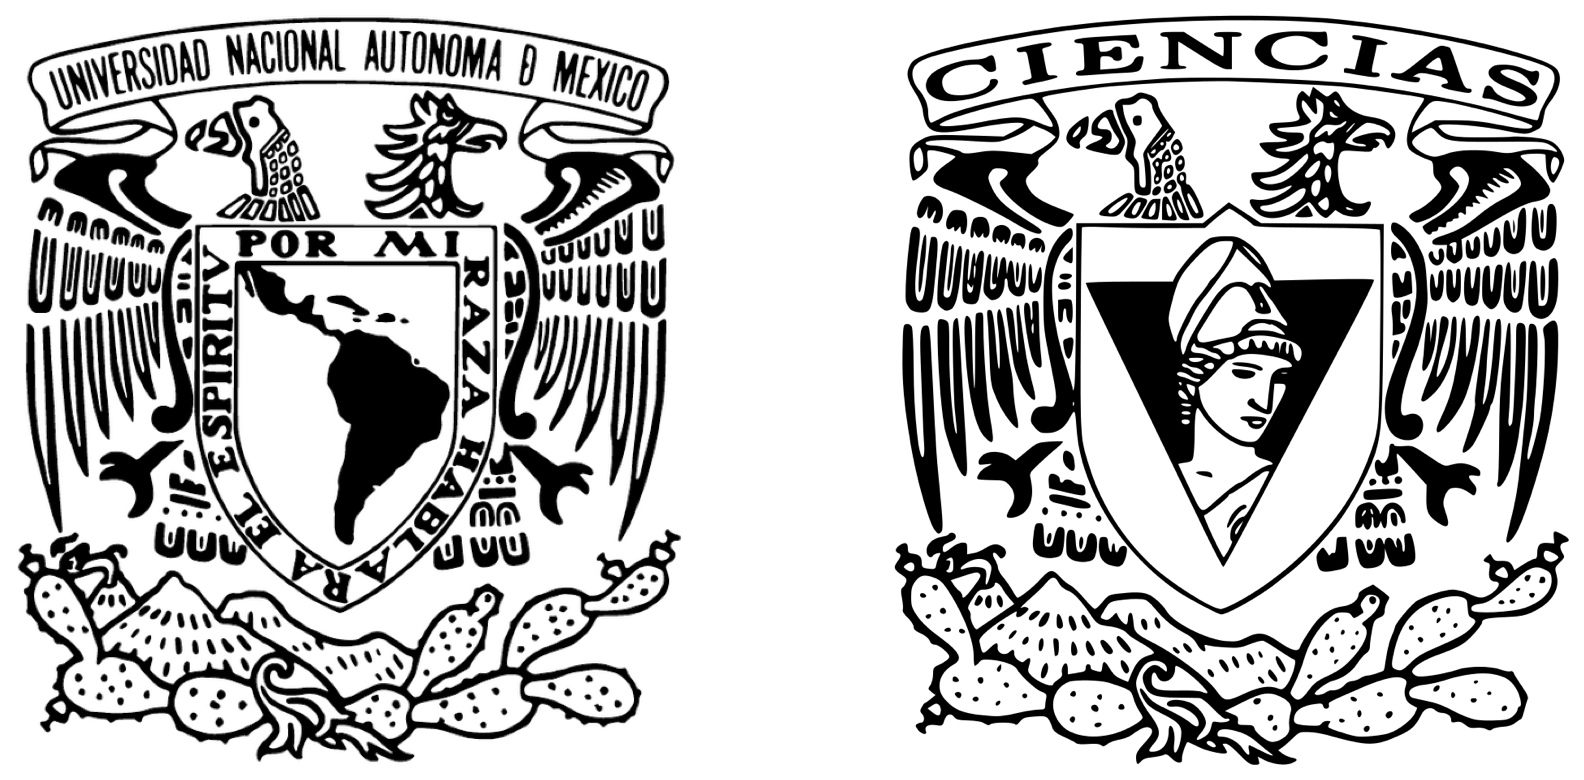
\includegraphics[scale=.1]{assets/img/logo.png}
    \end{center}

    \vspace{.8 cm}

    {\LARGE Tarea 1: \par}
    {\huge\bfseries Ejercicios \par}

    \vspace{0.5cm}
    \large{\itshape{Luis Erick Montes Garcia}} \small{ - 419004547}\\
    \large{\itshape{Hele Michelle Salazar Zaragoza}} \small{ - 316068895}


    \vfill

    Trabajo presentado como parte del curso de
    \textbf{Matematicas Aplicadas para las Ciencias II}
    impartido por el profesor \textbf{Juan Carlos Balleza}. \par
    \vspace{0.1cm}
    {\large Entrega 1 de Marzo 2019 \par}
    \footnotesize{\textbf{Link al código fuente:} git@github.com:lemg98/Matematicas-Aplicadas-II.git}
\end{titlepage}

    \begin{enumerate}
        %Ejercicio 1.
        \item 

        %Ejercicio 2.
        \item Sea la función vectorial $r (\overrightarrow{t}) = (4cos({t \over 2}),4sin({t \over 2}))$, donde $t \in [0,2\pi]$. A continuación responda lo siguiente:
        %Incisos del ejercicio 2.
        \begin{enumerate}
            %Inciso a
            \item Calcule los vectores de velocidad y aceleración.
            \\ Obtenemos la derivada de la función  $r (\overrightarrow{t})$ para obtener la {\bf velocidad}: 
            \begin{center}
                $r'(\overrightarrow{t}) = (-2sin({t \over 2}),2cos({t \over 2}))$ 
            \end{center}

            Obtenemos la derivada de la función $r'(\overrightarrow{t})$ para obtener la {\bf aceleración}:
            \begin{center}
                $r''(\overrightarrow{t}) = (-cos({t \over 2}),-sin({t \over 2}))$ \\
                \begin{tabular}{|c|c|c|} \hline 
                    t & velocidad & aceleración \\ \hline
                    $0$ & $(0,2) $ & $(-1,0)$  \\ \hline
                    $2\pi$ & $(-0.109,1.99)$ & $(-0.99,-0.054)$  \\ \hline
                \end{tabular}
            \end{center}

            %Inciso b
            \item Grafique la función vectorial, en el intervalo de $t$ indicado.
            \begin{center}
                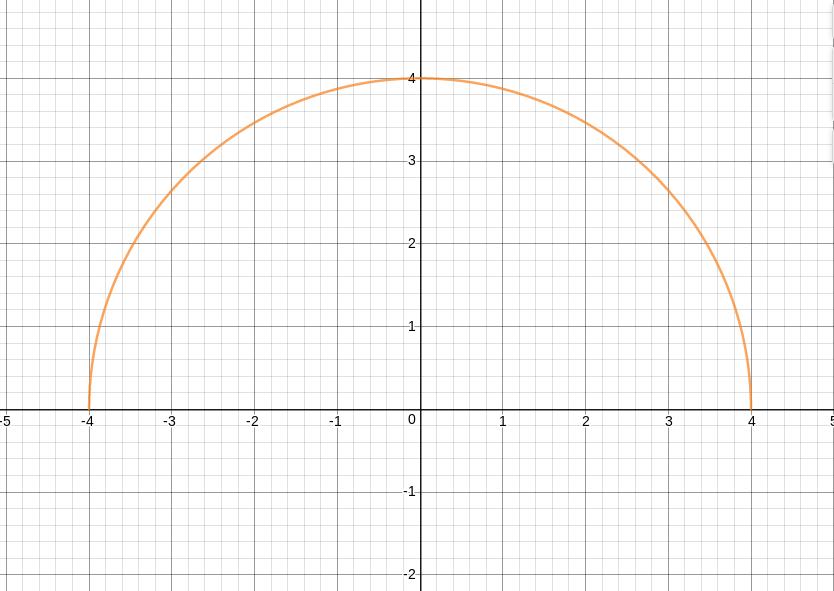
\includegraphics[scale=.3]{assets/img/ejercicio2(b).png}
            \end{center}
            %Inciso c
            \item En la gráfica de la función vectorial (inciso anterior), agregue los vectores de velocidad y aceleración en el instante $t = \pi$ 
            \begin{center}
                \begin{tabular}{|c|c|c|} \hline 
                    t & velocidad & aceleración \\ \hline
                    $\pi$ & $(-0.054,1.99) $ & $(-0.99,-0.02)$  \\ \hline
                \end{tabular}
                \\
                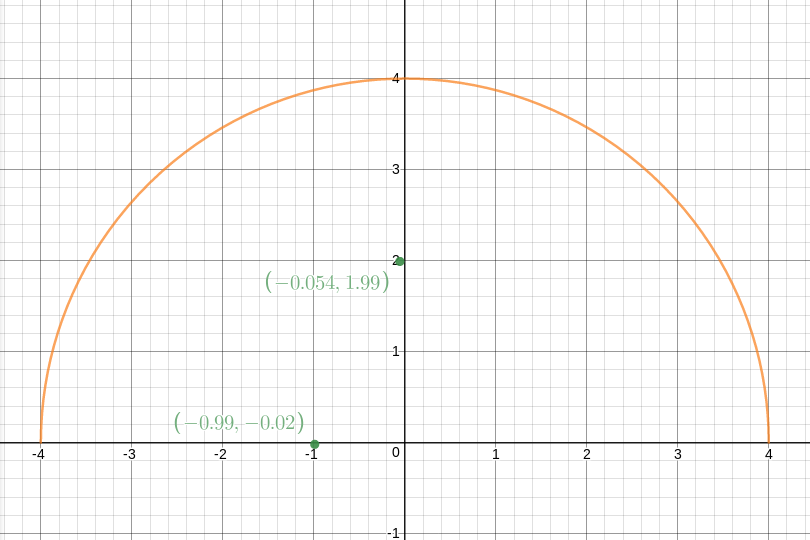
\includegraphics[scale=.3]{assets/img/ejercicio2(c).png}
            \end{center}

            %Inciso d
            \item Obtenga el ángulo entre los vectores velocidad y aceleración.
            \\ Decimos que el vector de velocidad es el vector $\overrightarrow{a}$ y que el vector de aceleración es \overrightarrow{b}. Para obtener el ángulo $\theta$ formamos un triángulo, siendo $\overrightarrow{a}-\overrightarrow{b}$ el lado opuesto al ángulo.
            \\ Aplicando ley de cosenos, tenemos que: \\
            $||\overrightarrow{a}-\overrightarrow{b}||^2=||\overrightarrow{a}||^2 + ||\overrightarrow{b}||^2-2||\overrightarrow{a}|| ||\overrightarrow{b}|| cos \theta $ \\
            Sustituímos: \\
        \end{enumerate}


        %Ejercicio 3.
        \item

        %Ejercicio 4.
        \item Proporcione la función vectorial $r(\overrightarrow{t})$, tal que cumpla las siguientes condiciones:
        %Incisos del Ejercicio 4.
        \begin{enumerate}
            %Inciso a
            \item $a(t)=(-1,-1,-1)$
            %Inciso b
            \item $v(0)=(0,0,0)$
            %Inciso c
            \item $r(0)=(10,10,10)$
        \end{enumerate}

        %Ejercicio 5.
        \item

        %Ejercicio 6.
        \item Considere la función vectorial $r(\overrightarrow{t})= ([cos t]^3,[sin t]^3)$. Responda lo siguiente:
        %Incisos del Ejercicio 6.
        \begin{enumerate}
            %Inciso a
            \item Obtenga el vector tangente unitario a la curva.
            %Inciso b
            \item Calcule la longitud de la curva para $t \in [0,{\pi \over 2}]$
        \end{enumerate}

        %Ejercicio 7.
        \item

        %Ejercicio 8.
        \item Obtenga la ecuación del círculo osculador para la función $y=sin x$ en el punto de coordenadas $({\pi \over 2},1)$. Proponga $r(\overrightarrow{t})$ a partir de la "parametrización trivial" de la función. Calcule lo siguiente: 
        %Incisos del Ejercicio 8.
        \begin{enumerate}
            \item $(\overrightarrow{T})$, $(\overrightarrow{N})$ y $k$.
        \end{enumerate}
        Haga una gráfica con la siguiente información:
        \begin{enumerate}
            \item La función $y=sin x$
            \item El círculo osculador y además localizar el punto de coordenadas $({\pi \over 2},1)$
            \item Los vectores $(\overrightarrow{T})$, $(\overrightarrow{N})$.
        \end{enumerate}

        %Ejercicio 9
        \item 


    \end{enumerate}





\end{document}